% \begin{wrapfigure}{r}{0.45\textwidth}  % r表示图片在右侧，0.5\textwidth表示图片宽度为文本宽度的50%
%     \centering
%     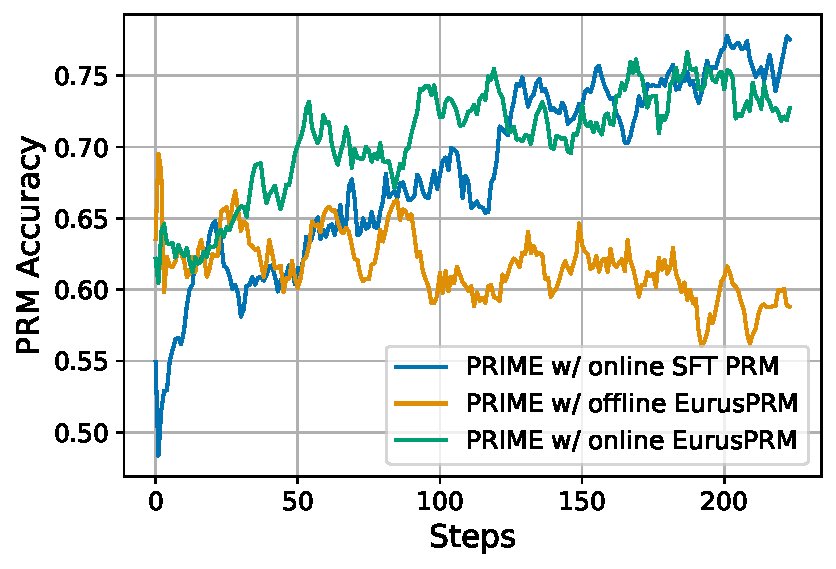
\includegraphics[width=\linewidth]{figures/images/prm_acc_online.pdf}  % 插入图片，宽度设置为wrapfigure环境的宽度
%     \caption{Classification accuracy of online and offline PRMs.} 
%     \label{fig:online_prm_acc}
% \end{wrapfigure}
\begin{wrapfigure}{r}{0.4\textwidth}
\vspace{-10pt} 
\centering
    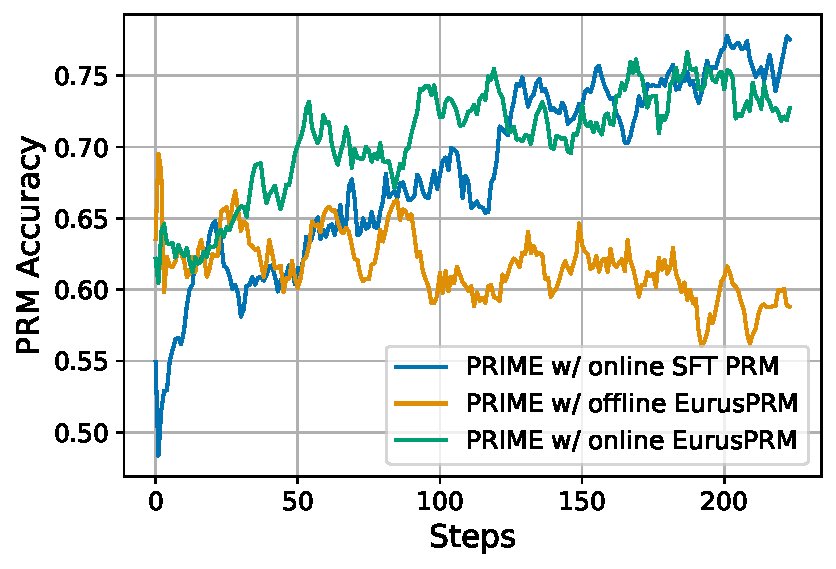
\includegraphics[width=\linewidth]{figures/images/prm_acc_online.pdf}
    \caption{\textbf{Impact of PRM online update.} Offline PRM is gradually been overoptimized while online PRMs achieve higher accuracy during training.}
    \label{fig:prm_acc_online}
    \vspace{-15pt} 
\end{wrapfigure}
